\chapter{Análise Exploratória} \label{cap:analise_exploratoria}

%\section{Comparação de funcionalidades} \label{subsec:comparacaofuncionalidades}

Foram selecionadas algumas funcionalidades muito comuns em aplicativos para serem comparadas entre iOS, Android e Ionic, com o objetivo de melhorar o embasamento para a tomada de decisão entre o desenvolvimento 
nativo e multiplataforma. Importante ressaltar que para o aplicativo Ionic utilizar os recursos do celular, tanto \textit{hardware} quanto \textit{software}, é sempre necessária a utilização de 
\textit{plugins} do Cordova, ou seja, sempre que um novo recurso for desenvolvido para um dispositivo, há um tempo de espera para a criação do \textit{plugin} necessário para utilizar o novo recurso, 
e se o \textit{plugin} for descontinuado, eventualmente poderá quebrar a aplicação e prejudicar a experiência do usuário. A seguir são apresentadas as funcionalidades e, em alguns casos, trechos de códigos minerados 
de repositórios públicos e criados pelos autores comentados para facilitar o entendimento das funcionalidades e diferenças entre cada plataforma e abordagem de desenvolvimento. 

\section{Funcionalidades analisadas}\label{sec:intro_analise_exp}

As funcionalidades alvo da análise e comparação são listadas a seguir e serão explicadas e comparadas nas Subseções~\ref{subsec:loginfb} à~\ref{subsec:facial}. 

\begin{itemize}
	\item Login com Facebook;
	\item Consumo de Web Services;
	\item Detecção de força do toque;
	\item Leitor Biométrico;
	\item Extração de metadados de arquivos;
	\item Envio de e-mail e SMS;
	\item Widgets;
	\item Assistentes Pessoais;
	\item Smartwatches;
	%\item Smart TV;
	\item Câmeras customizadas;
	\item Detecção facial;
\end{itemize}

\subsection{Login com Facebook} \label{subsec:loginfb}
%https://ionicthemes.com/tutorials/about/native-facebook-login-with-ionic-framework
Independente da plataforma, sempre deve haver um passo anterior ao desenvolvimento desta funcionalidade que é o registro do 
aplicativo a ser desenvolvido na plataforma para desenvolvedores do Facebook\footnote{\url{https://developers.facebook.com}}. O registro do aplicativo deve ser feito
para cada plataforma que se deseja atingir, por exemplo, iOS e Android, utilizando para isso, o nome do pacote do aplicativo em cada plataforma. 

Com esta estapa concluída, pode-se iniciar o desenvolvimento desta funcionalidade utilizando para isso o \textit{SDK} do Facebook para iOS e Android.
No caso do Ionic, existem alguns \textit{plugins} que podem ser utilizados, como por exemplo o \textit{\$cordovaOauth}\footnote{\url{http://ngcordova.com/docs/plugins/oauth/}}, disponível dentro do próprio ngCordova, 
que permite a conexão com vários provedores de serviços, tais como Google, Github, Facebook e Linkedin, por exemplo. 

Além desse, existem outros meios de se conectar aos provedores, por exemplo, utilizando o 
Firebase\footnote{\url{https://www.firebase.com}} do Google. Desta forma, é possível acessar os dados públicos do usuário como nome, e-mail e foto de perfil para realizar um cadastro e \textit{login} no aplicativo.
Em todas as três plataformas citadas (iOS, Android e Ionic), a complexidade é similar, havendo apenas diferenças inerentes a cada linguagem e plataforma. 

Vale ressaltar, que o \textit{login} com redes sociais, nada mais é do que a obtenção dos dados do usuário de uma plataforma terceira por meio do protocolo \textit{OAuth}, 
ou seja, não são criadas sessões a partir das plataformas terceiras, apenas os dados do usuário na outra plataforma são acessados para que não haja a necessidade do usuário informá-los novamente. A partir dos dados 
obtidos, o aplicativo se encarrega de realizar o cadastro e \textit{login} do usuário de acordo com as regras de negócio do aplicativo. 
As Figuras~\ref{fig:loginfb-ios} e~\ref{fig:loginfb-ionic} apresentam dois trechos de código no iOS e no Ionic para \textit{login} com o Facebook. No iOS foi utilizado o \textit{SDK} nativo do Facebook, 
já no Ionic, foi utilizado o \textit{Firebase}. 

\begin{figure}[H]
	\centering
	\includegraphics[width=1\textwidth]{codes/ios/loginfb}
	\caption[Requisição de dados do Facebook no iOS]{Requisição de dados do Facebook no iOS}
	\label{fig:loginfb-ios}
\end{figure}

\begin{figure}[H]
	\centering
	\includegraphics[width=1\textwidth]{codes/ionic/loginfb}
	\caption[Requisição de dados do Facebook no Ionic]{Requisição de dados do Facebook no Ionic. Fonte: Baseado em Github\protect\footnotemark}
	\label{fig:loginfb-ionic}
\end{figure}

\footnotetext{\url{https://github.com/fga-gpp-mds/2016.1-Partiu_frontend}}

Vale ressaltar que o \textit{plugin} do Cordova é genérico para vários provedores, ou seja, com o mesmo código é possível requisitar os dados em vários serviços distintos. Já nos \textit{SDKs} nativos, isso não ocorre.
Caso haja a necessidade de obtenção de dados de vários provedores, como por exemplo, no caso de \textit{login} com Facebook e Google, na abordagem nativa é preciso utilizar a \textit{SDK} do Facebook para iOS e Android
e a \textit{SDK} do Google para iOS e Android. O mesmo não ocorre no multiplataforma, pois com o mesmo \textit{plugin} é possível fazer a conexão com vários serviços apenas alterando uma \textit{string}, 
o que pode tornar o desenvolvimento mais simples que na abordagem nativa.

\subsection{Consumo de Web Services} \label{subsec:webservices}
Como o poder computacional dos dispositivos móveis, embora elevado, ainda não é comparável ao dos servidores, muitos aplicativos utilizam um modelo cliente/servidor, no qual
as operações mais custosas computacionamente são processadas no lado servidor e não no cliente. Além disso, a persistência dos dados da aplicação dificilmente é feita localmente nos dispositivos para evitar 
perdas de dados no caso de roubos, extravios ou danos ao aparelho, facilitar a migração para outros dispositivos e o uso em outras plataformas. Com isso, é necessário que os aplicativos estejam preparados para se 
comunicarem com \textit{Web Services}. Para realizar essa comunicação, cada plataforma oferece alguns meios nativos como classes e \textit{frameworks}, no entanto, existem \textit{frameworks} de terceiros que 
são muito utilizados e conhecidos na comunidade de desenvolvedores tanto para comunicar com os \textit{Web Services}, como para lidar com JSON e XML usados na comunicação entre aplicativo/servidor. 

No Android, existe o \textit{Volley}\footnote{\url{https://developer.android.com/training/volley/index.html}}, da própria Google para facilitar a envio e recebimento dos dados. Assim como no iOS, define-se o método da 
requisição, os parâmetros a serem enviados e dentro de um \textit{Listener} receber a resposta do servidor e tratar de acordo com as necessidades do aplicativo. Vale ressaltar que o \textit{Volley}, no momento da realização
deste trabalho, não é nativamente preparado para enviar dados, apenas receber, de maneira que deve-se criar uma classe customizada de requisição que adiciona os parâmetros a serem enviados na requisição e faz o tratamento da
resposta, para só então ser criada uma requisição que permite o envio de dados. No exemplo da Figura~\ref{fig:volley-android}, a classe criada chama-se \textit{CustomJSONObjectRequest} e sua implementação não se encontra 
na imagem.

Para realizar essa atividade no Ionic, o AngularJS dispõe do \textit{plugin ngResource} muito conhecido e utilizado para interação com \textit{web services}. Ele trás o objeto \textit{\$resource} que recebe uma 
\textit{URL} e parâmetros da requisição de maneira muito similar à abordagem nativa, apenas distinguindo em termos de linguagem e ambiente de programação. Assim como nas abordagens nativas, também é possível receber 
o retorno da requisição e tratá-lo dentro de uma \textit{\$promise}, cujo modo de uso se assemelha ao \textit{completion} do iOS e ao \textit{Listener} do Android. A Figura~\ref{fig:resource-ionic} apresenta um trecho 
de código implementando o consumo de um \textit{web service} privado no Ionic.

No iOS é possível realizar essa comunicação utilizando algumas classes nativas do sistema como por exemplo, \textit{NSURL}, \textit{NSData} e \textit{NSJSONSerialization}, informando uma \textit{URL} 
na qual o \textit{app} irá se conectar para receber ou enviar algum dado para o servidor, no entanto, toda essa comunicação e tratamento das respostas deverá ser feita manualmente. Para facilitar, existem alguns 
\textit{frameworks} terceiros como \textit{AlamoFire}\footnote{\url{https://github.com/Alamofire/Alamofire}} e \textit{SwiftyJSON}\footnote{\url{https://github.com/SwiftyJSON/SwiftyJSON}} 
que abstraem essa comunição e tratamento dos dados em JSON, respectivamente, tornando o código mais simples e limpo. Ao utilizá-lo, o programador apenas indica a \textit{URL}, o método da requisição 
(\textit{POST, GET, PUT, DELETE, etc}) e os parâmetros que deseja enviar ao servidor. Após isso, basta receber a resposta na forma de \textit{JSON} dentro de um \textit{completion} do \textit{Alamofire}, 
e utilizar os dados de acordo com as necessidades do aplicativo. Um trecho de código exemplificando o uso do \textit{AlamoFire} e \textit{SwiftyJSON} é apresentado na Figura~\ref{fig:alamofire-ios}.

\begin{figure}[H]
	\centering
	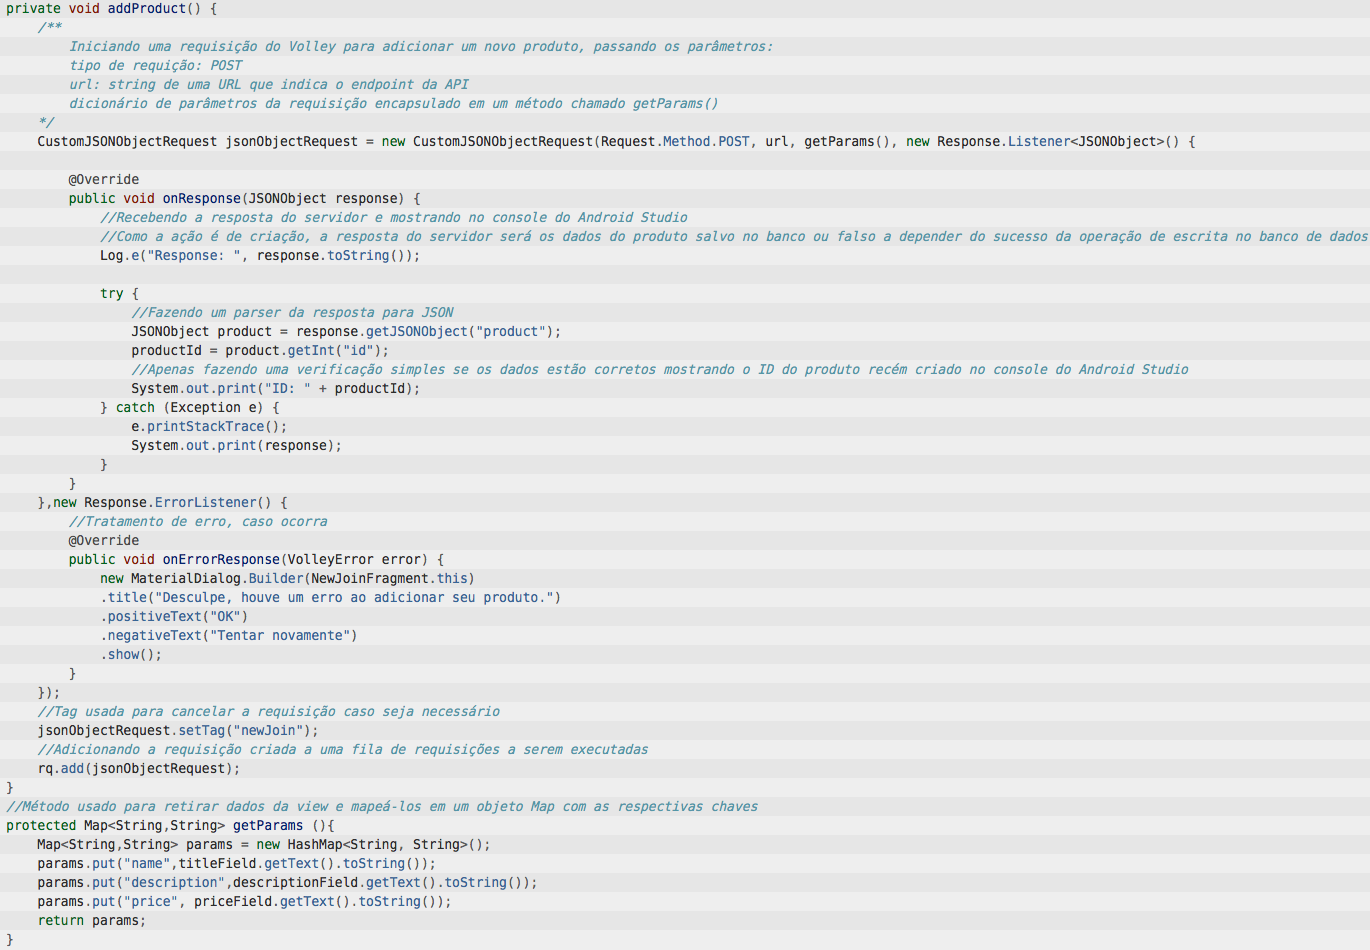
\includegraphics[width=0.95\textwidth]{codes/android/volley}
	\caption[Requisição utilizando Volley no Android]{Requisição utilizando Volley no Android}
	\label{fig:volley-android}
\end{figure}
\begin{figure}[H]
	\centering
	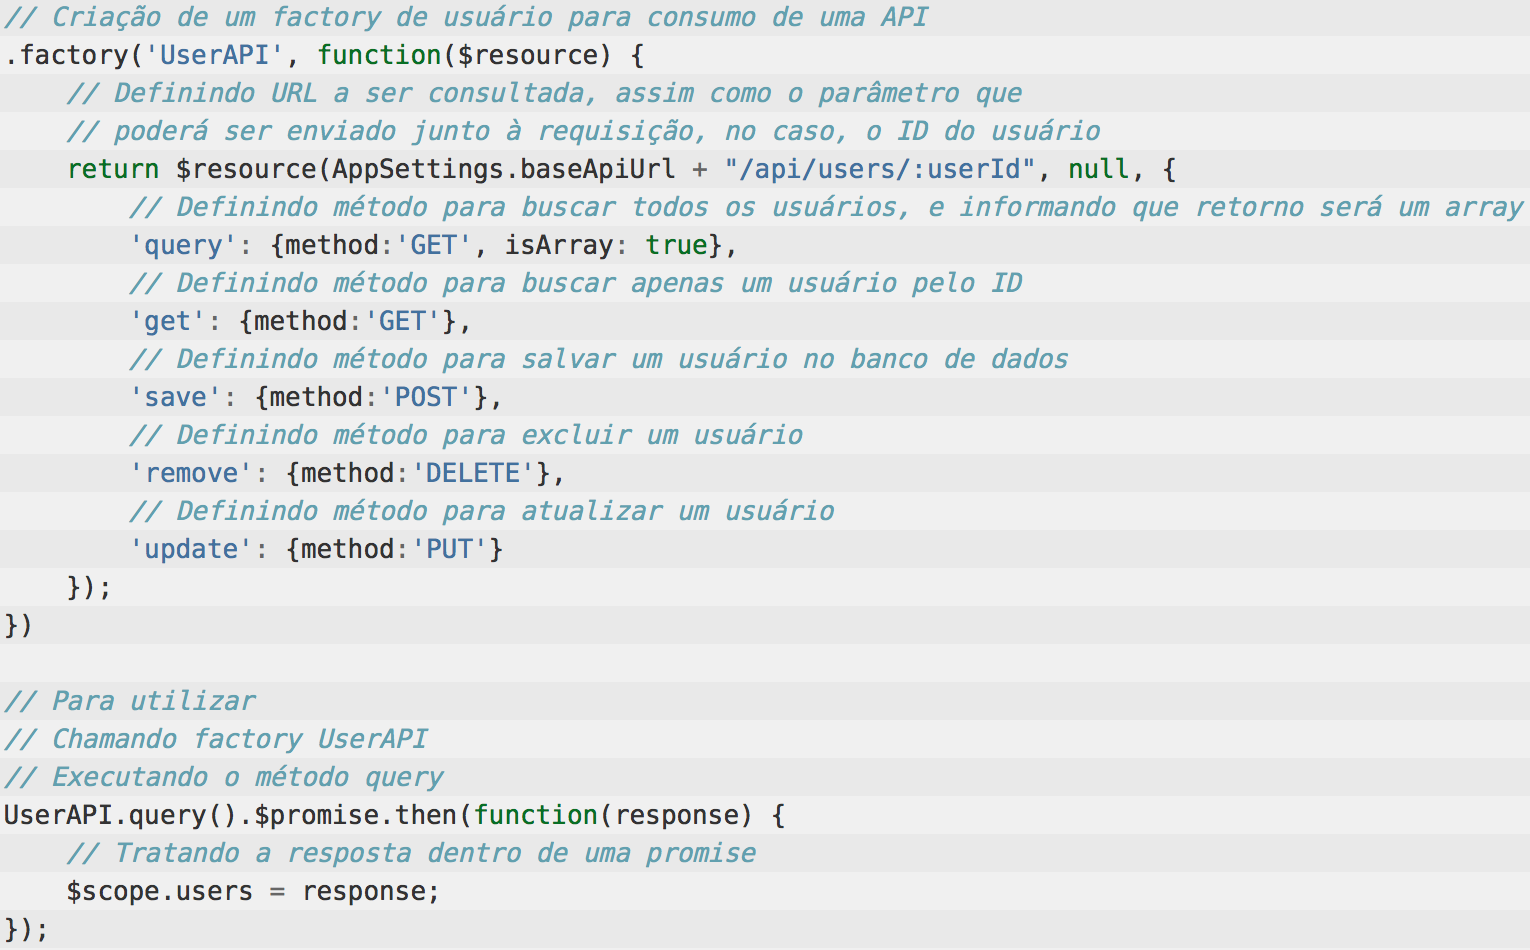
\includegraphics[width=1\textwidth]{codes/ionic/resource}
	\caption[Requisição utilizando o ngResource no Ionic]{Requisição utilizando o ngResource no Ionic. Baseado em Github\protect\footnotemark}
	\label{fig:resource-ionic}
\end{figure}
\footnotetext{\url{https://github.com/fga-gpp-mds/2016.1-Partiu_frontend}}
\begin{figure}[H]
	\centering
	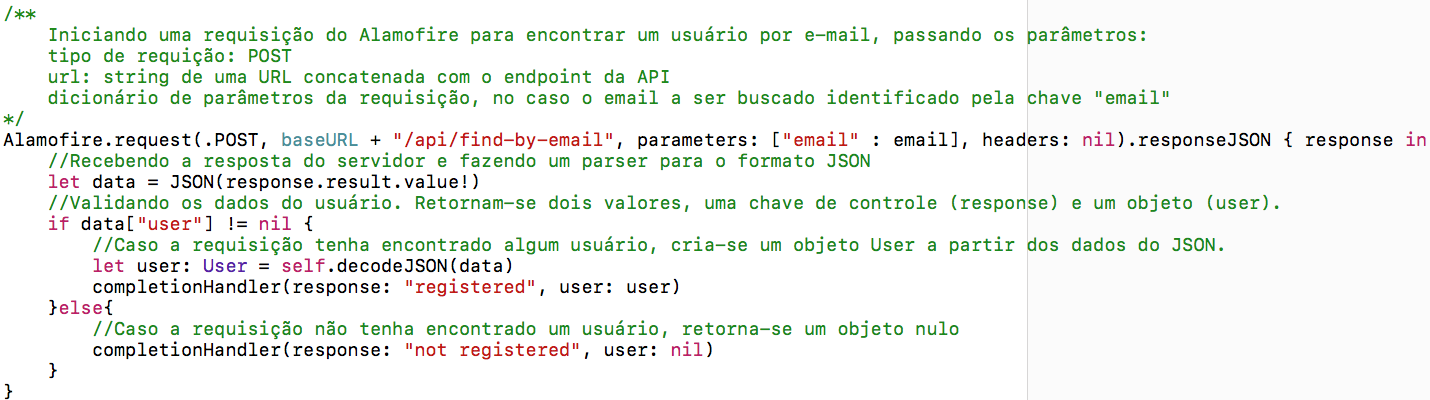
\includegraphics[width=1\textwidth]{codes/ios/alamofire}
	\caption[Requisição utilizando Alamofire e SwiftyJSON no iOS]{Requisição utilizando Alamofire e SwiftyJSON no iOS}
	\label{fig:alamofire-ios}
\end{figure} 

\subsection{Detecção de força do toque} \label{subsec:forcetouch}
Em 2015, alguns dispositivos móveis foram comercializados com uma tecnologia de detecção de pressão nas telas sensíveis ao toque. Primeiramente pela companhia chinesa Huawei e depois pela Apple, trata-se de um recurso 
capaz de identificar a quantidade de força que o usuário exerceu em um toque, o que abre o leque de possibilidades para novas funcionalidades nos aplicativos desenvolvidos. 
No iOS, é chamado de \textit{3DTouch} e por enquanto está disponível nos modelos de iPhone 6S ou superior. No Apple Watch e no novo MacBook, assim como no Mate S, da Huawei, é chamado apenas de \textit{Force Touch}, 
nome original da tecnologia. 
Vale ressaltar que o Android já possui a capacidade de ler a área de toque por meio de \textit{software} apenas, no entanto, o \textit{Force Touch} não é apenas a leitura de área de toque, mas sim da pressão do toque,
o que envolve \textit{hardware} e \textit{software}.

As Figuras~\ref{fig:3dtouch-ios} e~\ref{fig:forcetouch-ionic} apresentam trechos de código no iOS e no Ionic para utilização do \textit{3DTouch} criando \textit{Quick Actions}, uma funcionalidade do iOS que permite 
que o usuário aperte com mais força o ícone do aplicativo para ter algumas opções antes de entrar no aplicativo.

\begin{figure}[H]
	\centering
	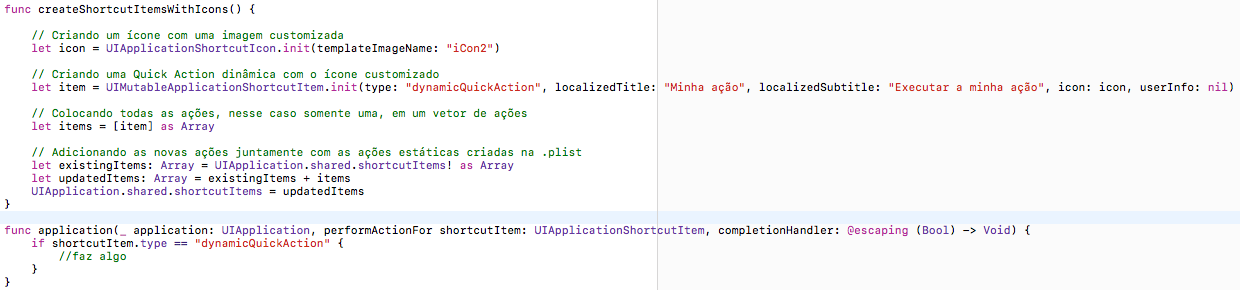
\includegraphics[width=1\textwidth]{codes/ios/3dtouch}
	\caption[Criando uma Quick Action com o 3DTouch no iOS.]{Criando uma Quick Action com o 3DTouch no iOS. Fonte: Baseado em Github\protect\footnotemark}
	\label{fig:3dtouch-ios}
\end{figure}
\footnotetext{\url{https://github.com/versluis/3D-Touch}}
\begin{figure}[H]
	\centering
	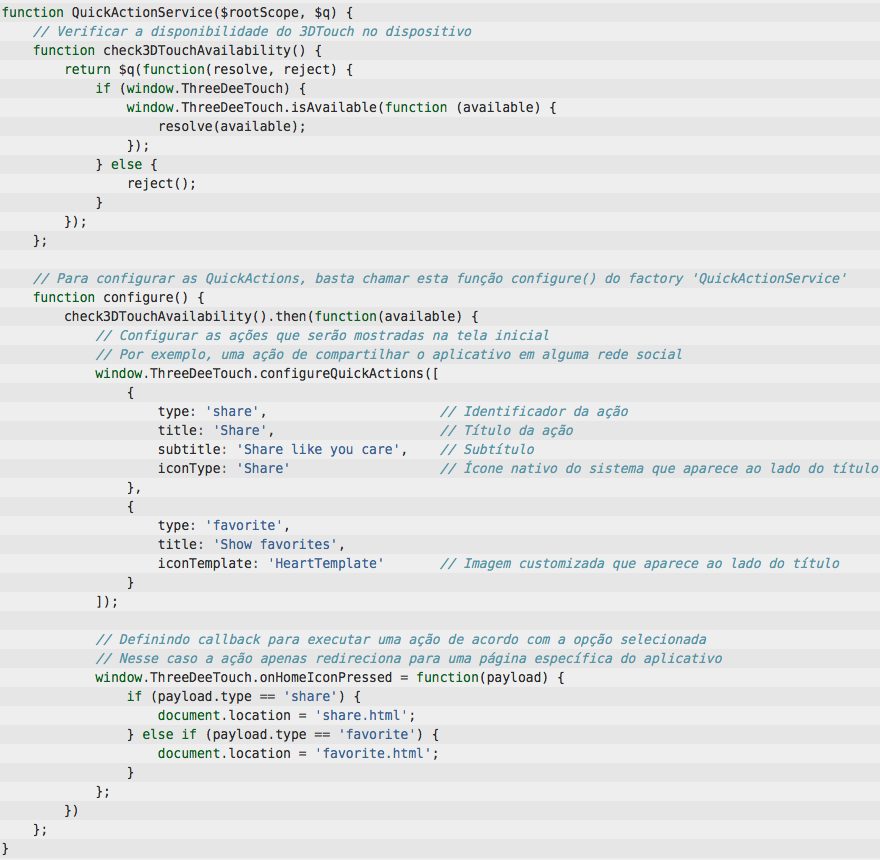
\includegraphics[width=1\textwidth]{codes/ionic/forcetouch}
	\caption[Criando uma Quick Action com o 3DTouch no Ionic]{Criando uma Quick Action com o 3DTouch no Ionic. Fonte: Baseado em Github\protect\footnotemark}
	\label{fig:forcetouch-ionic}
\end{figure}
\footnotetext{\url{https://github.com/ashteya/ionic-tutorial-quickactions}}

Em ambos os casos a implementação é simples apenas devendo-se considerar as diferenças entre plataformas e linguagens, no entanto, no caso do Ionic é necessária a utilização do 
\textit{plugin cordova-plugin-3dtouch}\footnote{\url{https://github.com/EddyVerbruggen/cordova-plugin-3dtouch}}. 

\subsection{Leitor Biométrico} \label{subsec:biometrico}
A preocupação por segurança dos dados e privacidade se intensificou, pois os dispositivos móveis agora possuem muitas informações pessoais como contatos, fotos, \textit{e-mails}, localização e até mesmo senhas, no entanto,
por serem móveis são mais fáceis de serem extraviados, furtados ou invadidos. Com isso, cada dispositivo possui seus próprios meios de autenticação e segurança, sendo a forma mais comum de segurança senhas alfanuméricas. 
Com o avanço da tecnologia presente nos dispositivos móveis, uma forma que se tornou comum para autenticação de usuário é a leitura biométrica, ou seja, reconhecimento de impressões digitais. Muitos \textit{smartphones} 
já possuem esse recurso adicionando ao celular uma camada extra de segurança e praticidade. 

Além do celular e dos dados pessoais do usuário, é possível que os dados de um aplicativo em específico sejam protejidos pelo mesmo recurso, ou seja, caso o aparelho seja encontrado desbloqueado, ainda não será possível 
ter acesso à todos os dados disponíveis dentro dele. Alguns aplicativos que se utilizam desse recurso são, por exemplo, bancos, diários, chaveiros eletrônicos e protetores de fotos. Nos dispositivos da Apple o recurso 
foi introduzido no iPhone 5 e foi chamado de \textit{Touch ID}, nos dispositivos Android, os aparelhos mais desenvolvidos de cada marca possuem o sensor biométrico. 

Como mencionando anteriormente, é possível proteger os dados de uma aplicação com o leitor biométrico. Para isso, o iOS dispõe do \textit{framework LocalAuthentication}, que permite que a aplicação solicite a leitura da 
digital, caso o aparelho possua o recurso, e compare com as impressões digitais cadastradas no dispositivo. Caso o dispositivo não possua o recurso, será requerida uma senha alfanumérica comum para desbloquear os dados do 
aplicativo. No Android, de maneira similar ao iOS, a partir da versão 6.0, foi introduzida uma nova \textit{API}, a \textit{Fingerprint Authentication}\footnote{\url{https://developer.android.com/about/versions/marshmallow/android-6.0.html}}, 
que permite utilizar o sensor biométrico dentro dos aplicativos. No Android, é preciso efetuar alguns passos, listados a seguir, antes de poder utilizar a autenticação biométrica. 

\begin{itemize}
	\item \textbf{Permissão}: É preciso adicionar uma permissão especial no arquivo \textit{Manifest} para que seja possível utilizar o sensor;
	\begin{itemize}
		\item \textit{<uses-permission android:name=``android.permission.USE\_FINGERPRINT''/>} 
	\end{itemize}
	\item \textbf{\textit{Container} de chaves}: É preciso acessar o \textit{container} de chaves do Android, para poder armazenar uma chave que será criada para a aplicação;
	\begin{itemize}
		\item \textit{KeyStore}: onde o sistema guarda todas as chaves de criptografia;
	\end{itemize}
	\item \textbf{Gerar uma chave}: Tendo acesso ao \textit{KeyStore}, é preciso gerar uma chave para a aplicação e então armazená-la no \textit{KeyStore};
\end{itemize}

As Figuras~\ref{fig:touchid-ios} e~\ref{fig:fingerprint-android} apresentam trechos de códigos que implementam a verificação biométrica em iOS e Android.

\begin{figure}[H]
	\centering
	\includegraphics[width=1\textwidth]{codes/ios/touchid}
	\caption[Implementação do Touch ID no iOS]{Implementação do Touch ID no iOS. Fonte: Baseado em AppCoda\protect\footnotemark}
	\label{fig:touchid-ios}
\end{figure}
\footnotetext{\url{https://www.appcoda.com/touch-id-api-ios8/}}
\begin{figure}[H]
	\centering
	\includegraphics[width=1\textwidth]{codes/android/fingerprint}
	\caption[Implementação da leitura biométrica no Android]{Implementação da leitura biométrica no Android. Fonte: Baseado em Google\protect\footnotemark}
	\label{fig:fingerprint-android}
\end{figure}
\footnotetext{\url{https://developer.android.com/samples/FingerprintDialog/index.html}}
%http://www.techotopia.com/index.php/An_Android_Fingerprint_Authentication_Tutorial
%https://github.com/googlesamples/android-FingerprintDialog

No Ionic também é possível utilizar a leitura biométrica nos aplicativos. No entanto, para utilizar esse recurso, é necessária a utilização de dois \textit{plugins} separados, um para iOS e um para Android, pois em 
cada plataforma a autenticação se dá de maneira específica e ainda não há um \textit{plugin} para ambas as plataformas. As Figuras~\ref{fig:finger-ios-ionic} e~\ref{fig:finger-android-ionic} apresentam dois trechos de 
códigos no Ionic implementando a leitura biométrica. Foram usados os seguintes \textit{plugins}, para iOS e Android, respectivamente:
\begin{itemize}
	\item \textbf{iOS}: \textit{cordova-plugin-touchid}\footnote{\url{https://github.com/leecrossley/cordova-plugin-touchid}};
	\item \textbf{Android}: \textit{cordova-plugin-android-fingerprint-auth}\footnote{\url{https://github.com/mjwheatley/cordova-plugin-android-fingerprint-auth}}; 
\end{itemize}
\begin{figure}[H]
	\centering
	\includegraphics[width=0.8\textwidth]{codes/ionic/touchid}
	\caption[Implementação da leitura biométrica para iOS no Ionic]{Implementação da leitura biométrica para iOS no Ionic. Fonte: Baseado em Github\protect\footnotemark}
	\label{fig:finger-ios-ionic}
\end{figure}
\footnotetext{\url{https://github.com/leecrossley/cordova-plugin-touchid}}
%https://www.thepolyglotdeveloper.com/2015/08/add-touch-id-authentication-to-your-ionic-framework-app/
\begin{figure}[H]
	\centering
	\includegraphics[width=0.8\textwidth]{codes/ionic/fingerprint}
	\caption[Implementação da leitura biométrica para Android no Ionic]{Implementação da leitura biométrica para Android no Ionic. Fonte: Baseado em Github\protect\footnotemark}
	\label{fig:finger-android-ionic}
\end{figure}
\footnotetext{\url{https://github.com/mjwheatley/cordova-plugin-android-fingerprint-auth}}

É possível criar aplicações que utilizem desse recurso nas duas abordagens, no entanto, de maneira geral, a implementação dessa funcionalidade é mais simples quando se trata do iOS, tanto nativo quanto multiplataforma, já 
que no Android são necessários alguns passos anteriores ao desenvolvimento. Em relação ao desenvolvimento no Android, o multiplataforma é mais simples que o nativo, em relação à complexidade e quantidade de código a ser 
desenvolvido.

\subsection{Extração de metadados de arquivos} \label{subsec:extracaometadata}
Em alguns casos, pode ser necessário a extração de metadados de algum arquivo específico, como uma imagem ou um áudio. No caso de uma imagem, podem ser retiradas informações como local, hora de criação e até mesmo 
dados climáticos no momento da captura da foto. No caso de um arquivo de áudio, é possível extrair o título do áudio, o autor ou artista, tempo de duração e álbum. Esses metadados podem ser usados para 
melhorar a experiência de uso do aplicativo fornecendo sugestões e funcionalidades mais próximas das necessidades reais do usuário, ou até mesmo para fazer filtros e buscas mais inteligentes nos dados que o 
aplicativo manuseia. 

Para extração de metadados no iOS existem classes nativas como a \textit{AVPlayerItem} e \textit{ALAssetsLibrary} para extração de metadados, respectivamente, de audio e imagens. No Android existe a 
classe \textit{MediaMetadataRetriever}, que lida com a extração de tipos variados de mídia. Em ambos os casos, iOS e Android, a implementação é simples, pois é preciso apenas seguir os métodos das classes 
utilizando constantes do sistema para indicar qual dado se deseja obter. Por exemplo, se o objetivo é obter a informação de título, no iOS, basta chamar pela \textit{string} ``title''. Já no Android, para o mesmo 
objetivo, basta chamar pela \textit{string} ``METADATA\_KEY\_TITLE''.

As Figuras~\ref{fig:metadata_audio-ios} e~\ref{fig:metadata_midia-android} apresentam trechos de códigos implementando a extração de metadados no iOS e no Android.

\begin{figure}[H]
	\centering
	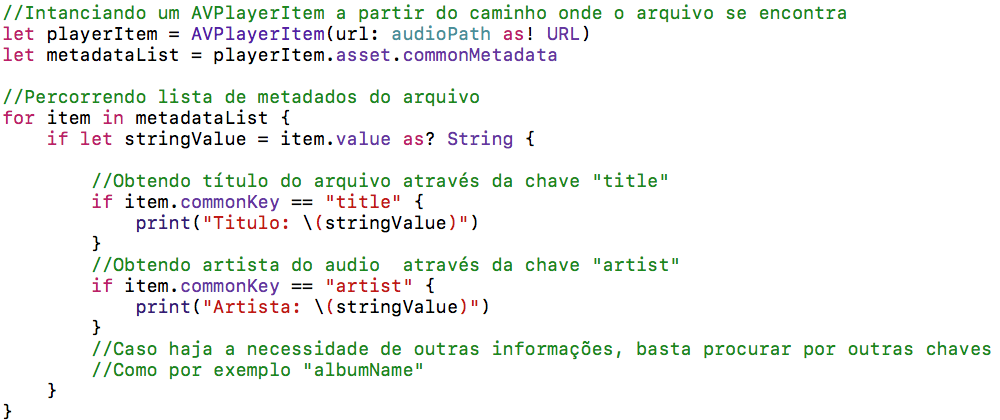
\includegraphics[width=0.8\textwidth]{codes/ios/metadata_audio}
	\caption[Extração de metadados de um arquivo áudio no iOS]{Extração de metadados de um arquivo áudio no iOS}
	\label{fig:metadata_audio-ios}
\end{figure}

\begin{figure}[H]
	\centering
	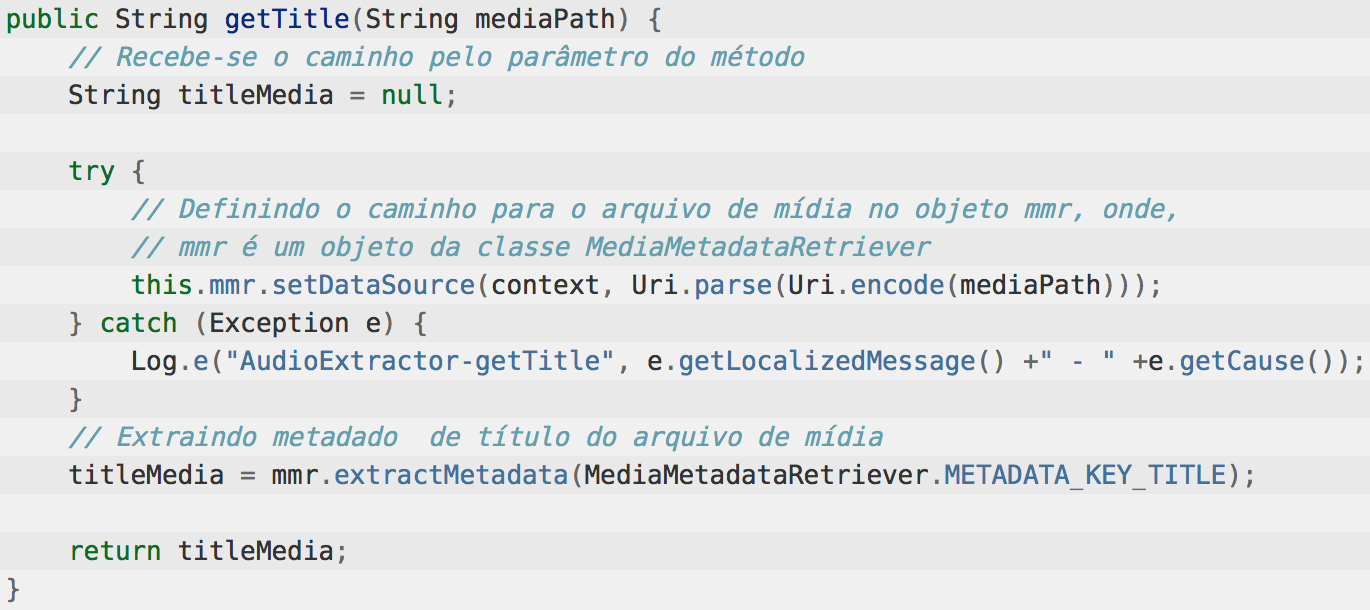
\includegraphics[width=0.8\textwidth]{codes/android/metadata_midia}
	\caption[Extração de metadados de um arquivo áudio no Android]{Extração de metadados de um arquivo áudio no Android. Baseado em Github\protect\footnotemark}
	\label{fig:metadata_midia-android}
\end{figure}

\footnotetext{\url{https://github.com/adorilson/MMUnB}}
%\begin{figure}[H]
%	\centering
%	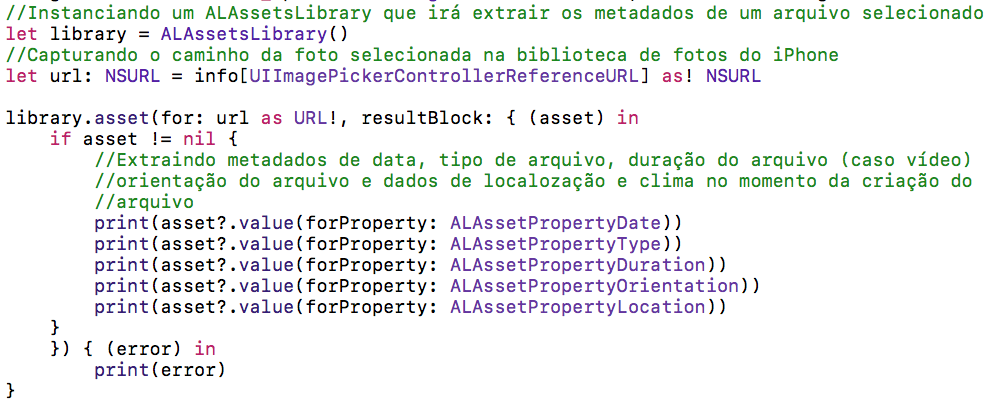
\includegraphics[width=1\textwidth]{codes/ios/metadata_video}
%	\caption[Trecho de código para extrair metadados de vídeo - iOS]{Trecho de código para extrair metadados de vídeo - iOS}
%	\label{fig:metadata_video-ios}
%\end{figure}

A extração de dados no Ionic pode ser realizada utilizando um \textit{plugin} do cordova chamado \textit{File}, utilizado para obter 
acesso aos arquivos e diretórios dos dispositivos. Na documentação do \textit{ngCordova} é apresentada a estrutura de pacotes do iOS e 
do Android, para auxiliar o desenvolvedor a acessar as pastas desejadas. É apresentada, também, uma lista de possíveis erros
que podem ocorrer durante o uso do plugin, como arquivo não encontrado, caminho inexistente, erro de \textit{encoding}, entre outros.
Com o plugin \textit{File} é possível obter as seguintes propriedades:
 
\begin{itemize}
	\item name: nome do arquivo seguido de sua extenção
	\item localURL: a url do arquivo, seguido de seu nome e extenção
	\item type: \textit{Internet media type} ou \textit{MIME type}, padrão usado na Internet para indicar um tipo de dado
	\item lastModifiedDate: data e hora da última modificação do arquivo
	\item size: tamanho do arquivo em bytes
\end{itemize}

Um exemplo de dados obtidos é apresentado na Figura~\ref{fig:metadata_result-ionic}. O código usado para 
obtenção destes dados é apresentado na Figura~\ref{fig:metadata_image-ionic}.
Para obtenção da duração de uma música ou um vídeo, é necessário o uso de outro  \textit{plugin} cordova chamado \textit{Media}.
Não foram encontrados plugins para obtenção de dados tão detalhados quanto os disponíveis no iOS e Android, como informações do autor 
e álbum de uma música ou a localização geográfica do local em que uma foto foi tirada.

\begin{figure}[H]
	\centering
	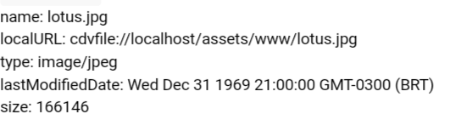
\includegraphics[width=1\textwidth]{codes/ionic/metadata_result}
	\caption[Apresentação dos metadados de uma imagem - Ionic]{Apresentação dos metadados de uma imagem - Ionic}
	\label{fig:metadata_result-ionic}
\end{figure}

\begin{figure}[H]
	\centering
	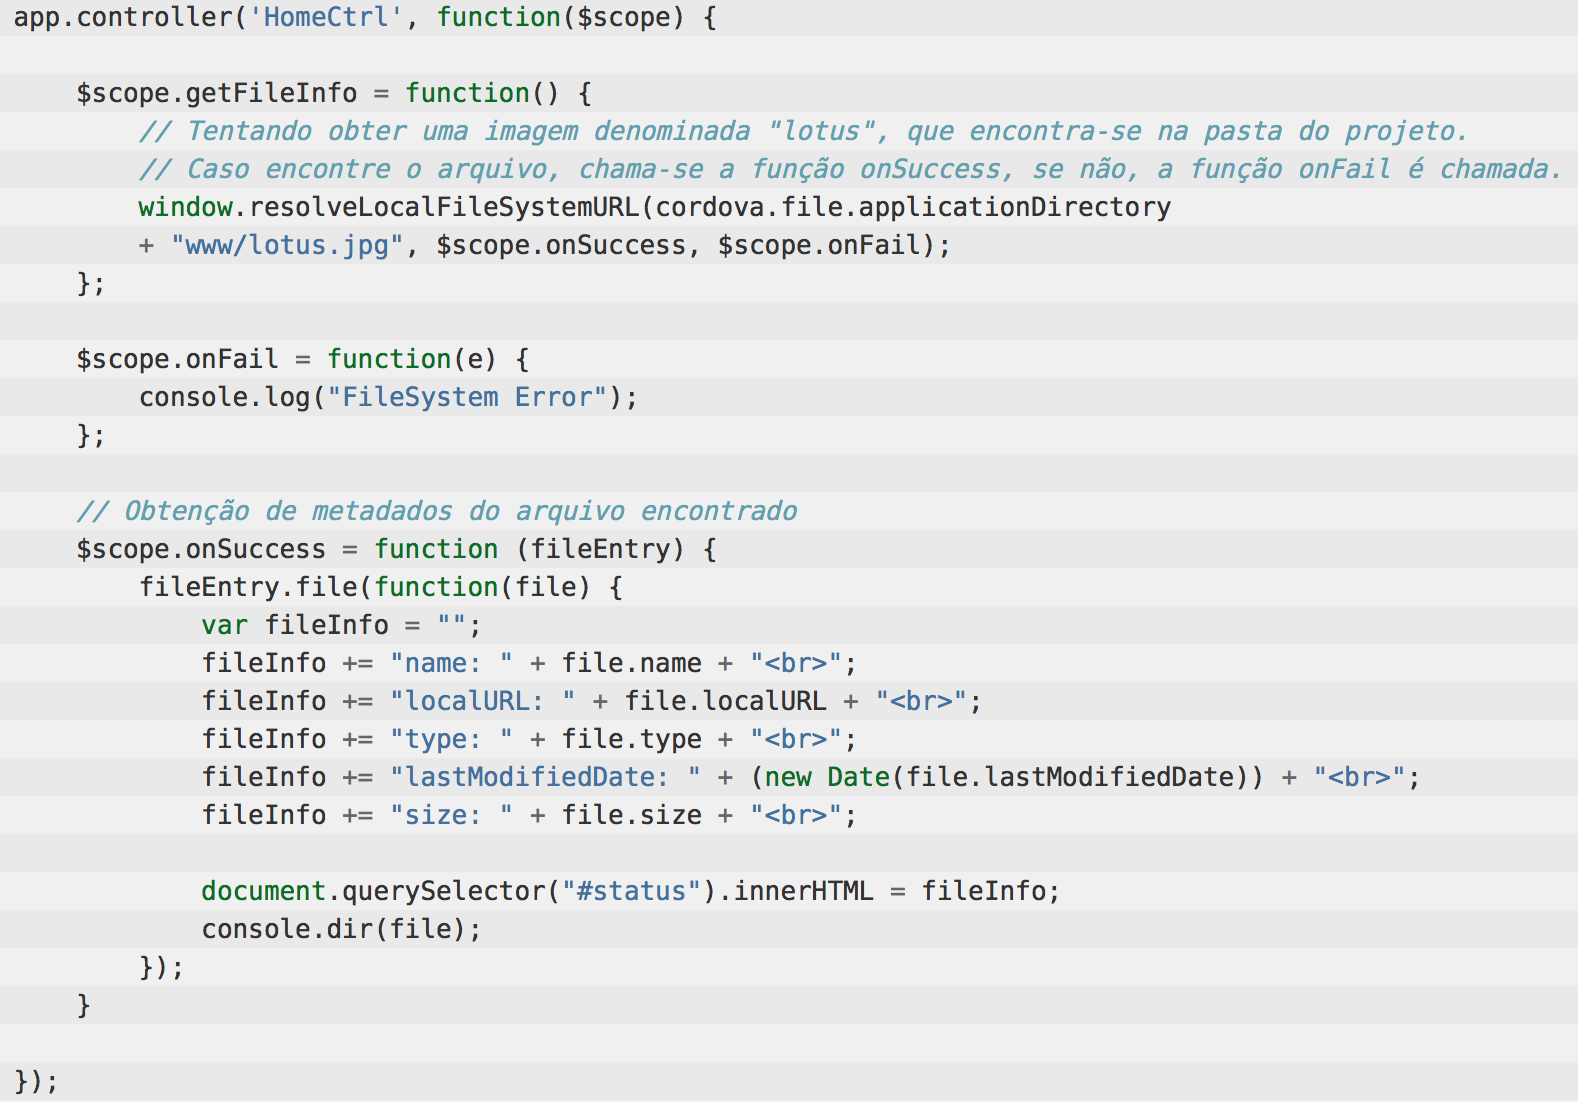
\includegraphics[width=1\textwidth]{codes/ionic/metadata_image}
	\caption[Extração de metadados de mídia no Ionic]{Extração de metadados de mídia no Ionic. Baseado em Github\protect\footnotemark}
	\label{fig:metadata_image-ionic}
\end{figure}
\footnotetext{\url{https://github.com/cfjedimaster/Cordova-Examples/tree/master/getfiledata}}

\subsection{Envio de e-mail e SMS} \label{subsec:emailsms}
Cada plataforma possui seus próprios \textit{frameworks} para incluir dentro do aplicativo a ser desenvolvido o mecanismo de envio de \textit{e-mails} ou mensagens de texto(\textit{SMS}), muito utilizados para compartilhar 
e divulgar informações do aplicativo ou até mesmo o próprio aplicativo e entrar em contato com a equipe de desenvolvimento do mesmo. Para utilizar desses recursos no Ionic, é possível utilizar o 
\textit{plugin cordova-plugin-email-composer}\footnote{\url{https://github.com/katzer/cordova-plugin-email-composer}} para ter acesso à interface padrão do sistema no qual o aplicativo está sendo executado para envio de 
\textit{e-mail}. De maneira similar, para o envio de \textit{SMS}, é possível utilizar o \textit{plugin cordova-sms-plugin}\footnote{\url{https://github.com/cordova-sms/cordova-sms-plugin}}. Tanto na abordagem nativa, 
quanto na multiplataforma o desenvolvimento é simples diferenciando apenas na linguagem e no ambiente. As Figuras~\ref{fig:email-ios} e~\ref{fig:email-ionic} apresentam dois trechos de código, no iOS e no Ionic, 
para o envio de \textit{e-mail}.
\begin{figure}[H]
	\centering
	\includegraphics[width=1\textwidth]{codes/ios/email}
	\caption[Envio de \textit{e-mail} no iOS]{Envio de \textit{e-mail} no iOS}
	\label{fig:email-ios}
\end{figure}
\begin{figure}[H]
	\centering
	\includegraphics[width=1\textwidth]{codes/ionic/email}
	\caption[Envio de \textit{e-mail} no Ionic]{Envio de \textit{e-mail} no Ionic. Baseado em Github\protect\footnotemark}
	\label{fig:email-ionic}
\end{figure}
\footnotetext{\url{https://github.com/katzer/cordova-plugin-email-composer}}

\begin{comment}
\subsection{Acessibilidade} \label{subsec:acessibilidade}
Não se pode deixar de lado uma grande parcela da população que possui algum tipo de deficiência na hora de planejar novos sistemas e 
aplicativos. Cada plataforma possui seus próprios recursos para auxiliar pessoas com 
deficiência a utilizar os \textit{smartphones} e também possuem \textit{SDKs} que os desenvolvedores podem utilizar para deixar os 
aplicativos usáveis para todos. No iOS existem muitos recursos disponíveis como VoiceOver, 
Ditado e a própria Siri\footnote{\url{http://www.apple.com/br/accessibility/ios}}. No Android exite o TalkBack, BrailleBack e Acesso 
por voz\footnote{\url{https://support.google.com/accessibility/android}}. 

Importante ressaltar que os aplicativos aliados às tecnologias presentes nos \textit{smartphones} podem ajudar pessoas com deficiência 
a serem incluídas socialmente, a viverem melhor e até mesmo ajudar na reabilitação 
já que alguns aplicativos são usados para fisioterapia e aprendizado diferenciado como no caso de pessoas com autismo ou daltonismo.

https://github.com/phonegap/phonegap-mobile-accessibility
https://github.com/driftyco/ionic/issues/4100

\end{comment} 
 
\subsection{\textit{Widgets}} \label{subsec:widgets}
\textit{Widgets} são atalhos que facilitam o acesso a algum programa. Vários dispositivos possuem esse recurso como computadores, camêras fotográficas, \textit{smartphones} e \textit{tablets}. Eles ajudam o usuário a 
realizar ações mais rapidamente e sem entrar necessáriamente em um programa ou aplicativo, sendo alguns dos mais comuns e práticos, o de agenda de eventos e informações climáticas.

Cada plataforma possui suas próprias maneiras de implementá-los, sendo no iOS apenas disponíveis na central de notificações do dispositivo e no Android sendo disponíveis tanto na tela inicial do aparelho quanto na central 
de notificações. A Figura~\ref{fig:widgets_sample} mostra exemplos de \textit{widgets} no iOS e Android respectivamente.

\begin{figure}[H]
	\centering
	\begin{minipage}{.5\textwidth}
		\centering
		\includegraphics[width=1\linewidth]{codes/ios/widget_eg}
	\end{minipage}%
	\begin{minipage}{.5\textwidth}
		\centering
		\includegraphics[width=1\linewidth]{codes/android/widget_eg}
	\end{minipage}
\caption[\textit{Widgets} no iOS (à esquerda) x \textit{Widgets} no Android (à direita).]{\textit{Widgets} no iOS (à esquerda) x \textit{Widgets} no Android (à direita).}
\label{fig:widgets_sample}
\end{figure}

Não é possível criar \textit{widgets} com Ionic e Cordova, pois utilizam \textit{HTML, CSS e JavaScript} embutidas em uma \textit{web view}, e fora dos aplicativos não há um \textit{browser} para renderizar o aplicativo 
feito no Ionic. O que poderia ser feito é criar o aplicativo multiplataforma e depois alterar os projetos nativamente em cada plataforma para adicionar o \textit{widget} que se deseja. Dessa forma, cada plataforma iria 
possuir códigos nativos para os respectivos \textit{widgets} além do código do aplicativo multiplataforma em si. Caso o \textit{widget} seja uma parte fundamental da aplicação, pode não ser uma boa ideia o 
desenvolvimento multiplataforma. 

\subsection{Assistentes Pessoais} \label{subsec:siri}
Os dispositivos móveis têm se tornado cada vez mais inteligentes e úteis para seus usuários. Funcionam como computadores, agendas, calendários, máquinas fotográficas, etc. Para atenderem ainda mais às necessidades de 
seus usuários, os dispositivos possuem em sua maioria inteligências artificiais, na forma de assistentes pessoais, criadas para auxiliar no uso dos \textit{smartphones, smartwatches} e \textit{smart TVs}. 
Na Apple, a assistente é conhecida como Siri, já no Android existem alguns aplicativos de terceiros que tentam criar uma assistente pessoal. O mais conhecido é Google Now, da própria Google, 
embora nesse caso ele não seja uma assitente pessoal, pois não possui traços de personalidade, ele apenas reconhece voz e responde a perguntas com muita eficiência.

Com a Siri é possível controlar o dispositivo, criando eventos, alarmes, lembretes, abrindo aplicativos e controlando eletrodomésticos, por exemplo, e fazer buscas variadas na \textit{internet}, com o Google Now 
apenas essa última opção está disponível. Durante a execução deste trabalho, foi lançado o primeiro celular inteiramente feito pela Google chamado de Pixel, que conta com o Google Assistant, uma evolução do Google Now 
para se tornar uma assistente pessoal. Com ele será possível também controlar o dispositivo assim como as outras assistentes de outras plataformas fazem. 

Durante a execução deste trabalho, a Apple lançou juntamente com a nova versão do sistema operacional, iOS 10, a \textit{API} da Siri para que aplicativos de terceiros possam interagir com a assistente pessoal tornando 
a experiência de uso dos aplicativos ainda mais intuitiva e prática. Ainda não há \textit{plugins} do Cordova que permitam o uso desse recurso, ou seja, caso haja a necessidade de utilizar a Siri, o multiplataforma ainda 
não é um opção viável. Vale ressaltar que existem alguns \textit{plugins} para utilizar o reconhecimento de voz e transcrever em texto\footnote{\url{https://github.com/api-ai/api-ai-cordova}} o que foi dito, no entanto, 
isso não é o mesmo que interagir com a Siri. O Google Assistant ainda não está disponível em outros dispositivos além do Pixel da Google e não existem \textit{SDK} nativo ou \textit{plugins} de terceiros para utilizá-lo. 
Com isso, por enquanto, ainda não é possível desenvolver aplicativos multiplataforma integrados com as assistentes pessoais mais utilizadas.

\subsection{\textit{Smartwatches}} \label{subsec:facial}

Além de \textit{smartphones} e \textit{tablets}, estão começando a ficar populares os dispositivos \textit{vestíveis} como relógios inteligentes. Isso implica em mais plataformas para dominar 
e mais possibilidades de aplicativos e funcionalidades para desenvolver. Um dos \textit{smartwatches} mais populares, atualmente, é o Apple Watch. Lançado com um sistema operacional próprio derivado do iOS, o WatchOS, 
por enquanto, funciona como uma extensão dos aplicativos criados para iPhone, ou seja, adiciona funcionalidades de rápida interação ao relógio para que não seja necessário interagir com o celular a todo momento.

Caso haja a necessidade de criar um aplicativo que suporte o Apple Watch, pode-se optar por desenvolver multiplataforma também, pois já existem \textit{plugins}
\footnote{\url{https://github.com/leecrossley/cordova-plugin-apple-watch}} do Cordova para realizar a integração entre o aplicativo multiplataforma e a extensão para Apple Watch. No entanto, o \textit{plugin} 
citado só funciona enquanto o aplicativo no iPhone está rodando. Quando, por algum motivo, o aplicativo deixa de rodar o \textit{plugin} não consegue mais se comunicar com o relógio podendo prejudicar a experiência 
de uso do aplicativo. Com isso, pode não ser uma boa ideia utilizar funcionalidades que precisam de atualização em tempo real, por exemplo, que recebe dados de um servidor, pois se o aplicativo no iPhone não 
estiver rodando, o relógio não conseguirá se comunicar e pegar os dados mais recentes, fazendo com 
que apresente dados desatualizados, prejudicando a experiência de uso.

Vale ressaltar que o aplicativo no Apple Watch deve ser feito nativamente, diretamente no Xcode. O \textit{plugin} apenas fornece um meio para que o \textit{app} multiplataforma do iPhone possa transmitir e receber 
dados do \textit{app} do relógio, mas não é possível criar a interface e controladoras do relógio via multiplataforma, pois o Apple Watch não possui um navegador (\textit{WebView}) para interpretar o JavaScript assim 
como o iPhone. Então, deve ser feito o aplicativo utilizando Cordova e Ionic, por exemplo, para o iPhone, e depois criar o \textit{app} no Xcode para Apple Watch e então utilizar um \textit{plugin} para realizar a 
comunicação entre os dois aplicativos.  

Se o aplicativo planeja utilizar muitos recursos do Apple Watch, como frequencímetro, pedômetro e acelerômetro, como aplicativos voltados para a área da saúde por exemplo, pode ser melhor desenvolver nativamente,
pois o foco não estará sendo em desenvolver o aplicativo para várias plataformas, mas sim para um dispositivo específico. Com isso, pode-se aproveitar melhor todos os recursos do relógio e todos os benefícios da integração
do mesmo com o iPhone.

Caso o aplicativo já exista, ainda que seja multiplataforma, é possível desenvolver o aplicativo para o relógio, no entanto, a comunicação entre o iPhone e o relógio não será perfeita no multiplataforma como é no nativo, 
o que implica em limitar as funcionalidades do aplicativo no relógio para não prejudicar a experiência do usuário, podendo até mesmo fazer com que não valha a pena investir tempo e esforço na criação do aplicativo para
relógio. Cabe ressaltar que também já existem \textit{plugins}\footnote{\url{https://github.com/tgardner/cordova-androidwear}} do Cordova para Android Wear, os \textit{smartwatches} que rodam Android.

\begin{comment}
	

\subsection{\textit{Smart TV}} \label{subsec:tv}
Assim como os \textit{smartwatches}, também existem outros dispositivos que estão ficando cada vez mais inteligentes e conectados à \textit{internet}, como por exemplo, os aparelhos de televisão. Alguns já vêm
com um sistema inteligente de fábrica, no entanto, é possível acoplar centrais multimídia ao televisor por meio de cabos \textit{HDMI} e à \textit{internet} por meio de \textit{Wi-fi} ou conexão \textit{ethernet}, 
deixando-os mais inteligentes e úteis. Alguns exemplos comerciais são a Apple TV, da Apple, e o Chrome Cast do Google. É possível desenvolver aplicativos para os televisores, aproveitando ao máximo os recursos de 
áudio e vídeo do aparelho, tornando a experiência com televisão ainda mais imersiva e prática. 

Cada plataforma possui sua própria \textit{SDK} para desenvolvimento dos aplicativos para TV e embora já existam \textit{plugins} do Cordova para lidar com o desenvolvimento de aplicativos para Apple TV e Chrome Cast, o aplicativo criado não será portado para ambas as plataformas (iOS e Android) e para cada nova funcionalidade que cada TV desenvolver, deverá ser desenvolvido o \textit{plugin} para utilizá-la, ao passo que 
no desenvolvimento nativo, será possível utilizar o máximo de cada plataforma sempre, respeitando sempre os guias de usabilidade de cada uma. 

Caso a equipe de desenvolvimento já possua conhecimentos em \textit{HTML, CSS, JavaScript} e \textit{Cordova}, pode ser vantajoso desenvolver o aplicativo multiplataforma, considerando o tempo de densenvolvimento, por 
mais que tenha que ser feito em dois projetos distintos, um para iOS e um para Android, pois a \textit{expertise} da equipe pode compensar. No entanto, ainda será necessário possuir conta de desenvolvedor, um computador com 
MacOS e Xcode para subir o aplicativo iOS para a loja, por isso caso já haja alguém com experiência no ambiente e plataforma da Apple, desenvolver nativamente seria mais recomendado nas atuais circunstâncias. 

Assim como os \textit{smartwatches}, as TVs possuem guias de estilo e usabilidade muito diferentes dos dispositivos móveis, pois possuem tamanhos de telas e recursos de \textit{hardware} e \textit{software} completamente 
distintos, ou seja, o desenvolvimento multiplataforma está cada vez mais difícil por ter que, cada vez mais, abarcar um gama de dispositivos muitos diferentes, variando em tamanhos que vão de uma polegada e meia a
até mais de 100 polegadas e sistemas operacionais, com \textit{SDKs}, \textit{frameworks}, \textit{hardware} e recursos próprios de cada plataforma. 
\end{comment}

\subsection{Câmeras customizadas} \label{subsec:customcamera}

Um dos recursos mais utilizados nos \textit{smartphones} é a câmera fotográfica. Muitos usuários definem o aparelho a ser adquirido com base na capacidade da camêra, com isso muitos aplicativos aproveitam para 
oferecer mais funcionalidades que os aplicativos de camêras nativos dos dispositivos. Funcionalidades como filtros de imagens, edição de vídeos, câmera lenta, integração com redes sociais e, em alguns casos, os aplicativos 
são uma rede social em si. Caso o aplicativo tenha a necessidade de camêras customizadas é possível desenvolvê-lo multiplataforma utilizando alguns \textit{plugins} para o Cordova, por exemplo o 
\textit{cordova-plugin-camera-preview}\footnote{\url{https://github.com/cordova-plugin-camera-preview/cordova-plugin-camera-preview}}.

Tanto o iOS quanto o Android fornecem suporte para a criação de camêras customizadas de acordo com as necessidades dos aplicativos. No iOS é possível utilizar o \textit{framework AVFoundation} para identificar as camêras 
presentes no dispositivo e utilizá-las de acordo com as regras de negócio do aplicativo. É possível criar interfaces completamente customizadas com quaisquer funcionalidades que a equipe de desenvolvimento seja capaz de 
implementar. Assim como no iOS, no Android também é possível criar camêras customizadas utilizando o \textit{framework android.hardware.camera2}.

\subsection{Detecção facial} \label{subsec:facial}
A detecção facial é uma tecnologia usada em uma grande variedade de aplicações que identificam rostos humanos em imagens. Detectar rostos humanos e extrair traços faciais é uma importante funcionalidade com diversas 
possibilidades de aplicações, tais como reconhecimento facial para autenticação de usuário e videoconferências. %\cite{wong_efficient_2000}.

A plataforma iOS possui um processador de imagens nativo denominado \textit{CIDetector}, capaz de identificar faces em imagens e vídeos. O \textit{SDK} do Android possui uma \textit{API} para detecção facial, 
a \textit{Face Detection}, capaz de detectar faces em imagens.

É possível realizar o processo de detecção facial como o uso de bibliotecas não nativas, como o OpenCV, uma biblioteca livre e multiplataforma amplamente utilizada para processamento de imagens. Com ela é possível 
não apenas a detecção, como também o reconhecimento facial.

Outro exemplo de tecnologia multiplataforma para detecção facial é o Beyond Reality Face NXT, um \textit{SDK} que oferece suporte a aplicações iOS nativas e a aplicações multiplataformas desenvolvidas com o 
uso de \textit{actionscript}.% \cite{site_beyond_2016}.

O Mobile Vision, da Google, é uma \textbf{API} que possibilita a detecção facial em fotos, vídeos e \textit{streams} ao vivo, tanto em plataformas Android, como em iOS.

O Cordova não apresenta bibliotecas próprias para a realização de detecção facial, sendo necessário o uso de bibliotecas externas. O Scanbot é um exemplo de \textit{SDK} que pode ser utilizado junto ao Cordova e 
possibilita detecção de documentos e de faces em tempo real, porém não é totalmente compatível com iOS e não é uma ferramenta gratuita. %\cite{gmbh_javascript_2016}

\section{Consolidação dos resultados} \label{sec:compa_conclu}

\begin{comment}
\textcolor{red}{\textit{Resumo as funcionalidades, só para facilitar a leitura e entendimento}}
\begin{itemize}
	\item \textbf{Login com Facebook}: Simples, possível com todas as abordagens, não é um fator tão decisivo assim...
	\item \textbf{Consumo de Web Services}: Simples, possível com todas as abordagens, não é um fator tão decisivo assim...
	\item \textbf{Leitor Biométrico}: Simples, possível com todas as abordagens, não é um fator tão decisivo assim, iOS mais fácil que Android, nas duas abordagens...
	\item \textbf{Extração de metadados de arquivos}: Simples, possível com todas as abordagens, não é um fator tão decisivo assim, no entanto, nativo possui mais informações a serem extraídas...
	\item \textbf{Envio de e-mail e SMS}: Simples, possível com todas as abordagens, não é um fator tão decisivo assim... (DAR OLHADA NO ANDROID DISSO E PROCURAR UM CÓDIGO)
	\item \textbf{Widgets}: Pode vir a ser bastante complexo pois tem implementaçoes e interpretações completamente distintas no iOS e no Android, não é possível desenvolver no multiplataforma, pode ser bastante decisivo...
	\item \textbf{Assistentes pessoais}: Não é possivel integrar os apps multiplataforma com a assistente pessoal do iOS e o Android nem possui uma nativa ainda, pode ser bastante decisivo...
	\item \textbf{SmartWatches}: Para Apple Watch os plugins multiplataforma são fracos e só funcionam enquanto o app esta aberto (integração entre relogio e celular é fraca), app do relogio deve ser feito nativamente, 
	existem plugins para Android (nao foram testados por falta de android wear, tempo), pode ser bastante decisivo...
	\item \textbf{Smart TVs}: Existem plugins para iOS e para Android, mas nao para os dois ao mesmo tempo, isso implica em desenvolver dois projetos separadamente de qualquer forma. Se a equipe tem expertise em tecnologias 
	web, pode ser vantajoso desenvolver multiplataforma para se aproveitar dessa expertise, no entanto, ainda será preciso computador com MacOS e Xcode, se o alvo for a TV, pode ser bastante decisivo 
	\item \textbf{Câmeras customizadas}: É possível desenvolver aplicativos multiplataforma com cameras customizadas, porem quanto maior a customização mais dificil o desenvolvimento, tanto para nativo quanto para 
	multiplataforma, entao cabe a avaliacao da expertise da equipe para saber o que é melhor, pode ser muito decisivo...
	\item \textbf{Detecção facial}: É possível desenvolver multiplataforma pois exsitem frameworks e plugins para isso, deve-se considerar a performance do aplicativo e uso da internet, pode ser muito decisivo...
\end{itemize}
\end{comment}

As funcionalidades \textbf{Login com Facebook}, \textbf{Consumo de Web Services}, \textbf{Envio de e-mail e SMS} e uso do \textbf{Leitor Biométrico} podem ser desenvolvidas tanto na abordagem nativa quanto na 
multiplataforma, sem ressalvas, não causando influência na escolha entre abordagens.

Para a realização de \textbf{extração de metadados de arquivos de mídia}, é possível utilizar ferramentas multiplataforma, porém há restrições quanto à obtenção dos dados, visto que alguns deles 
puderam ser obtidos apenas no desenvolvimento nativo.

A criação de \textbf{Widgets} ainda não é possível com o uso de ferramentas multiplataforma baseadas em soluções \textit{web}, como o Cordova.

Para o uso de \textbf{assistentes pessoais}, como a Siri e o Google Assistant, é necessário o uso de tecnologias nativas.

Não é possível criar aplicativos para \textbf{SmartWatches}, como o Apple Watch, utilizando o Cordova. O que pode-se fazer é criar o aplicativo de celular, utilizando tecnologias multiplataforma, o aplicativo do relógio, 
feito nativamente, e a comunicação do aplicativo com o relógio usando tecnologias multiplataforma, porém esta comunicação terá restrições, por exemplo o aplicativo do relógio só conseguirá trocar informações se o 
aplicativo do celular estiver aberto, o que não é necessário na solução totalmente nativa.

É possível desenvolver aplicativos multiplataforma com \textbf{câmeras customizadas}, porém quanto maior a customização, mais difícil o desenvolvimento, tanto para nativo quanto para multiplataforma, cabendo analisar 
a \textit{expertise} da equipe para saber qual abordagem escolher.

Para realização de \textbf{detecção facial} em fotos, vídeos e em tempo real, é possível utilizar ferramentas multiplataformas, porém muitas das \textit{APIs} disponibilizadas para isso não são gratuitas ou apresentam 
algum tipo de restrição, como funcionamento em apenas uma das plataformas, Android ou iOS. Já no desenvolvimento nativo, as próprias plataformas disponibilizam \textit{APIs} que possibilitam detecções faciais.

\begin{comment}
Para a criação de aplicativos para \textbf{SmartTVs}, há no Cordova \textit{plugins} para iOS e para Android, mas não para os dois ao mesmo tempo, isso implica em desenvolver dois projetos separadamente de qualquer forma. Se 
a equipe tem \textit{expertise} em tecnologias \textit{web}, pode ser vantajoso desenvolver multiplataforma para se aproveitar disso, no entanto, ainda será preciso um computador com MacOS e Xcode. Portanto se o foco for 
desenvolver este tipo de aplicativo é mais vantajoso utilizar as tecnologias nativas disponiblizadas pelas plataformas, aproveitando, assim, o máximo de desempenho e capacidade dos dispositivos de TV.
\end{comment}

\section{Opinião dos especialistas} \label{sec:questionario}
Com o propósito de confrontar a opinião dos especialistas da área de desenvolvimento móvel com os resultados obtidos empiricamente, foi elaborada uma série de afirmações baseadas 
nas informações obtidas na primeira etapa da análise exploratória. Além das afirmações de caráter técnico, foram elaboradas outras duas para avaliar a percepção geral dos especialistas em relação ao desenvolvimento 
multiplataforma. Considerando as funcionalidades analisadas, foi abordada a viabilidade de desenvolvimento das mesmas no ambiente multiplataforma. Os especialistas poderiam expressar as suas opiniões de acordo com as 
opções listadas a seguir.

\begin{itemize}
	\item \textbf{Concordo}: funcionalidade em questão pode ser desenvolvida no ambiente multiplataforma, sem ressalvas;
	\item \textbf{Concordo, mas há limitações quando comparado ao desenvolvimento nativo}: funcionalidade em questão pode ser desenvolvida no ambiente multiplataforma, com ressalvas;
	\item \textbf{Discordo}: funcionalidade em questão não pode ser desenvolvida no ambiente multiplataforma;
	\item \textbf{Não sei opinar}: não sabe se é possível desenvolver a funcionalidade no ambiente multiplataforma;
	\item \textbf{Outros}: resposta aberta, caso o profissional queira dar uma opinião mais detalhada a respeito da funcionalidade; 
\end{itemize}

O questionário, bem como os gráficos de análise dos resultados encontram-se no Apêndice~\ref{apen:questionario}.

\subsection{Análise dos dados coletados} \label{subsec:analisedadosquestionario}
Avaliando as respostas dadas ao questionário, observou-se que a percepção dos especialistas para as funcionalidades de \textbf{Login com Facebook}, \textbf{Consumo de \textit{Web Service}} e \textbf{envio de \textit{e-mail} e SMS}
coincidiu com os resultados obtidos na análise exploratória. Tais funcionalidades já estão muito difundidas entre os desenvolvedores, além disso, possuem baixo grau de complexidade de implementação no ambiente nativo. 
Além da experiência própria, esses podem ter sido os principais motivos para que tenham sido analisadas como passíveis de serem implementadas no ambiente multiplataforma.

Para as funcionalidades de \textbf{Leitor Biométrico}, \textbf{\textit{Widgets}} e \textbf{Assistentes Pessoais} a maior parte dos especialistas não soube opinar. Por serem funcionalidades não essenciais, isto é, 
funcionalidades que se ausentes, não impedem o funcionamento do aplicativo, nem todos os especialistas conhecem ou já tiveram experiência desenvolvendo alguma delas, dificultando o julgamento. 

Em relação ao desenvolvimento de aplicativos para \textbf{\textit{Smartwatches}}, a maioria não soube opinar. Por ser uma tecnologia recente no mercado e não popularizada no país, é possível que os especialistas não 
tenham experiência e nem interesse neste nicho de aplicações. Para os que opinaram, cerca de 70\% acha que não é possível a criação de aplicativos para os mesmos utilizando tecnologias multiplataforma, coincidindo com 
os resultados obtidos na análise exploratória. Quanto à comunicação entre o aplicativo para \textbf{\textit{Smartwatch}} e o aplicativo no celular, apenas 5\% dos especialistas responderam de acordo com os dados da análise 
exploratória, ou seja, concordam que há restrições na comunicação entre ambos os aplicativos. Isso reforça a falta de conhecimento e interesse dos especialistas neste tipo de tecnologia.

No que diz respeito à funcionalidade de \textbf{Detecção Facial}, metade dos especialistas foram equivocados em suas respostas, discordando ou concordando totalmente com a possibilidade do uso deste recurso no ambiente 
multiplataforma. Na realidade, a implementação deste recurso e possível, porém com limitações, de acordo com os dados obtidos na análise exploratória.  

Quanto à possibilidade de criação de \textbf{Câmeras Customizadas}, mais da metade dos especialistas não sabem que esta funcionalidade pode ser implementada sem limitações no ambiente multiplataforma, conforme os dados 
obtidos na análise exploratória.

Considerando a necessidade de \textbf{extração de metadados de arquivos de mídia}, apenas 25\% dos especialistas estão de acordo com o que foi obtido na análise exploratória, isto é, é possível a extração de metadados, porém
com limitações nos dados obtidos.

Foi questionado se a abordagem multiplataforma pode ser utilizada em qualquer cenário de desenvolvimento móvel, onde 75\% dos especialistas discordaram. Os demais concordaram com a afirmação, no entanto, acreditam que 
poderão ocorrer algum tipo de restrição no decorrer do desenvolvimento do aplicativo. Também foi questionado se com a evolução das ferramentas multiplataforma, elas não apresentam mais limitações quando comparadas com as 
nativas, onde 80\% dos especialistas discordaram.

Foi percebido que muitos especialistas não souberam opinar sobre muitas das questões anteriores e mesmo assim nenhum acredita que o desenvolvimento multiplataforma pode ser usado em qualquer cenário sem restrição. Além 
disso, a grande maioria acredita que as ferramentas são limitadas quando comparadas às nativas. De fato, o multiplataforma não é a melhor opção para todos os cenários e ainda apresenta limitações quando comparado à 
abordagem nativa, porém os especialistas compactuam com essas ideias mesmo sem conhecer as reais capacidades do ambiente multiplataforma, indicando um possível prejulgamento da abordagem.